% Balance sheet diagrams for SFC monetary operations

\begin{figure}[htbp]
\centering
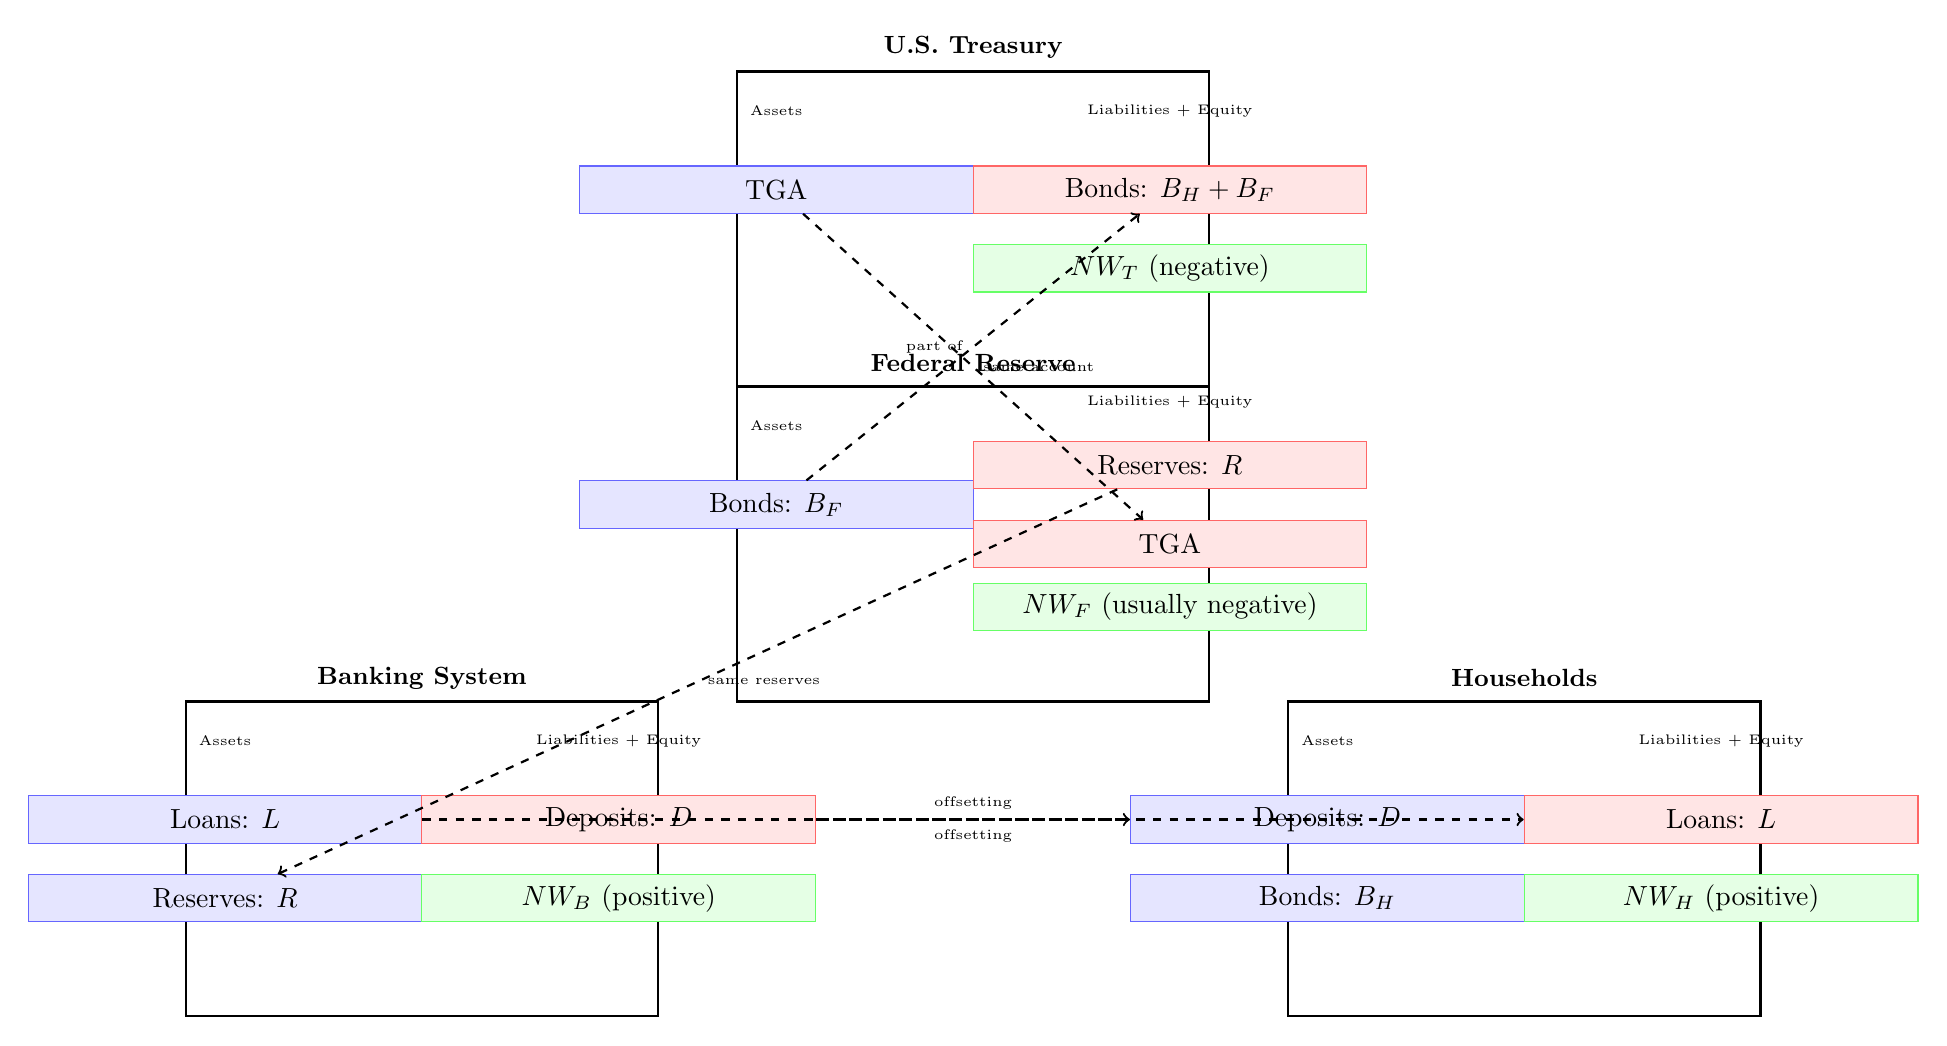
\begin{tikzpicture}[
    sector/.style={rectangle, draw=black, thick, minimum width=6cm, minimum height=4cm},
    asset/.style={rectangle, draw=blue!60, fill=blue!10, minimum width=5cm, minimum height=0.6cm},
    liability/.style={rectangle, draw=red!60, fill=red!10, minimum width=5cm, minimum height=0.6cm},
    equity/.style={rectangle, draw=green!60, fill=green!10, minimum width=5cm, minimum height=0.6cm},
    label/.style={font=\small\bfseries}
]

% Treasury
\node[sector] (treasury) at (0,6) {};
\node[label] at (0,8.3) {U.S. Treasury};
\node[asset] (tga) at (-2.5,6.5) {TGA};
\node[liability] (bonds) at (2.5,6.5) {Bonds: $B_H + B_F$};
\node[equity] (treasuryeq) at (2.5,5.5) {$NW_T$ (negative)};
\node[label, font=\tiny] at (-2.5,7.5) {Assets};
\node[label, font=\tiny] at (2.5,7.5) {Liabilities + Equity};

% Federal Reserve
\node[sector] (fed) at (0,2) {};
\node[label] at (0,4.3) {Federal Reserve};
\node[asset] (fedbonds) at (-2.5,2.5) {Bonds: $B_F$};
\node[liability] (reserves) at (2.5,3) {Reserves: $R$};
\node[liability] (tgaliab) at (2.5,2) {TGA};
\node[equity] (fedeq) at (2.5,1.2) {$NW_F$ (usually negative)};
\node[label, font=\tiny] at (-2.5,3.5) {Assets};
\node[label, font=\tiny] at (2.5,3.8) {Liabilities + Equity};

% Banking System
\node[sector] (banks) at (-7,-2) {};
\node[label] at (-7,0.3) {Banking System};
\node[asset] (loans) at (-9.5,-1.5) {Loans: $L$};
\node[asset] (bankreserves) at (-9.5,-2.5) {Reserves: $R$};
\node[liability] (deposits1) at (-4.5,-1.5) {Deposits: $D$};
\node[equity] (bankeq) at (-4.5,-2.5) {$NW_B$ (positive)};
\node[label, font=\tiny] at (-9.5,-0.5) {Assets};
\node[label, font=\tiny] at (-4.5,-0.5) {Liabilities + Equity};

% Households
\node[sector] (households) at (7,-2) {};
\node[label] at (7,0.3) {Households};
\node[asset] (deposits2) at (4.5,-1.5) {Deposits: $D$};
\node[asset] (hhbonds) at (4.5,-2.5) {Bonds: $B_H$};
\node[liability] (hhloans) at (9.5,-1.5) {Loans: $L$};
\node[equity] (hheq) at (9.5,-2.5) {$NW_H$ (positive)};
\node[label, font=\tiny] at (4.5,-0.5) {Assets};
\node[label, font=\tiny] at (9.5,-0.5) {Liabilities + Equity};

% Connections
\draw[->, thick, dashed] (tga) -- (tgaliab) node[midway, right, font=\tiny] {same account};
\draw[->, thick, dashed] (fedbonds) -- (bonds) node[midway, left, font=\tiny] {part of};
\draw[->, thick, dashed] (reserves) -- (bankreserves) node[midway, right, font=\tiny] {same reserves};
\draw[->, thick, dashed] (deposits1) -- (deposits2) node[midway, above, font=\tiny] {offsetting};
\draw[->, thick, dashed] (loans) -- (hhloans) node[midway, below, font=\tiny] {offsetting};

\end{tikzpicture}
\caption{Four-Sector Balance Sheet Structure. Dashed lines show offsetting entries across sectors. Private Net Financial Wealth = $R + B_H$ = $-$(Treasury NW + Fed NW).}
\label{fig:balance-sheets}
\end{figure}

\begin{figure}[htbp]
\centering
\begin{tikzpicture}[
    node distance=1.5cm and 2cm,
    process/.style={rectangle, rounded corners, draw=black, thick, minimum width=3cm, minimum height=1cm, align=center},
    flow/.style={->, thick},
    label/.style={font=\small}
]

% Horizontal Money Flow
\node[process, fill=blue!20] (bankloan) {Bank extends\\loan $+\Delta L$};
\node[process, fill=blue!20, right=of bankloan] (depositcreate) {Deposit created\\$+\Delta L$};
\node[label, above=0.5cm of bankloan, font=\bfseries] {Horizontal Money (Endogenous)};
\draw[flow] (bankloan) -- (depositcreate) node[midway, above, font=\footnotesize] {simultaneous};
\node[below=0.3cm of depositcreate, font=\footnotesize, align=center] {$\Delta(\text{Private NFW}) = 0$\\Loan \& deposit offset};

% Vertical Money Flow
\node[process, fill=green!20, below=3cm of bankloan] (treasury) {Treasury\\spends $+G$};
\node[process, fill=green!20, right=of treasury] (privatesector) {Private sector\\receives deposits $+G$};
\node[label, above=0.5cm of treasury, font=\bfseries] {Vertical Money (Exogenous)};
\draw[flow] (treasury) -- (privatesector) node[midway, above, font=\footnotesize] {via Fed};
\node[below=0.3cm of privatesector, font=\footnotesize, align=center] {$\Delta(\text{Private NFW}) = +G$\\Net financial asset created};

% QE Operation
\node[process, fill=orange!20, below=3cm of treasury] (qe1) {Households hold\\bonds $B_H$};
\node[process, fill=orange!20, right=of qe1] (qe2) {Fed buys bonds\\pays with reserves};
\node[process, fill=orange!20, right=of qe2] (qe3) {Households hold\\reserves $R$};
\node[label, above=0.5cm of qe1, font=\bfseries] {Quantitative Easing (Asset Swap)};
\draw[flow] (qe1) -- (qe2);
\draw[flow] (qe2) -- (qe3);
\node[below=0.3cm of qe2, font=\footnotesize, align=center] {$\Delta(\text{Private NFW}) = 0$\\Portfolio rebalancing only};

\end{tikzpicture}
\caption{Three Types of Monetary Operations. Horizontal money (bank lending) creates offsetting assets and liabilities. Vertical money (fiscal operations) changes net financial wealth. QE is a portfolio swap that preserves net wealth.}
\label{fig:operations}
\end{figure}
